\item  %2 points #32 Aug 2017
%this question doesn't seem right to me
On the axes below, sketch a possible function $p(x) =(x - a)(x -   b)(x + c)$, 
where $a$, $b$, and $c$ are positive, $a > b$, and $p(x)$ has a positive $y$-intercept of $d$. 
Label all intercepts.

\vspace{0.5 in}
\begin{figure}[!ht]
    \centering
    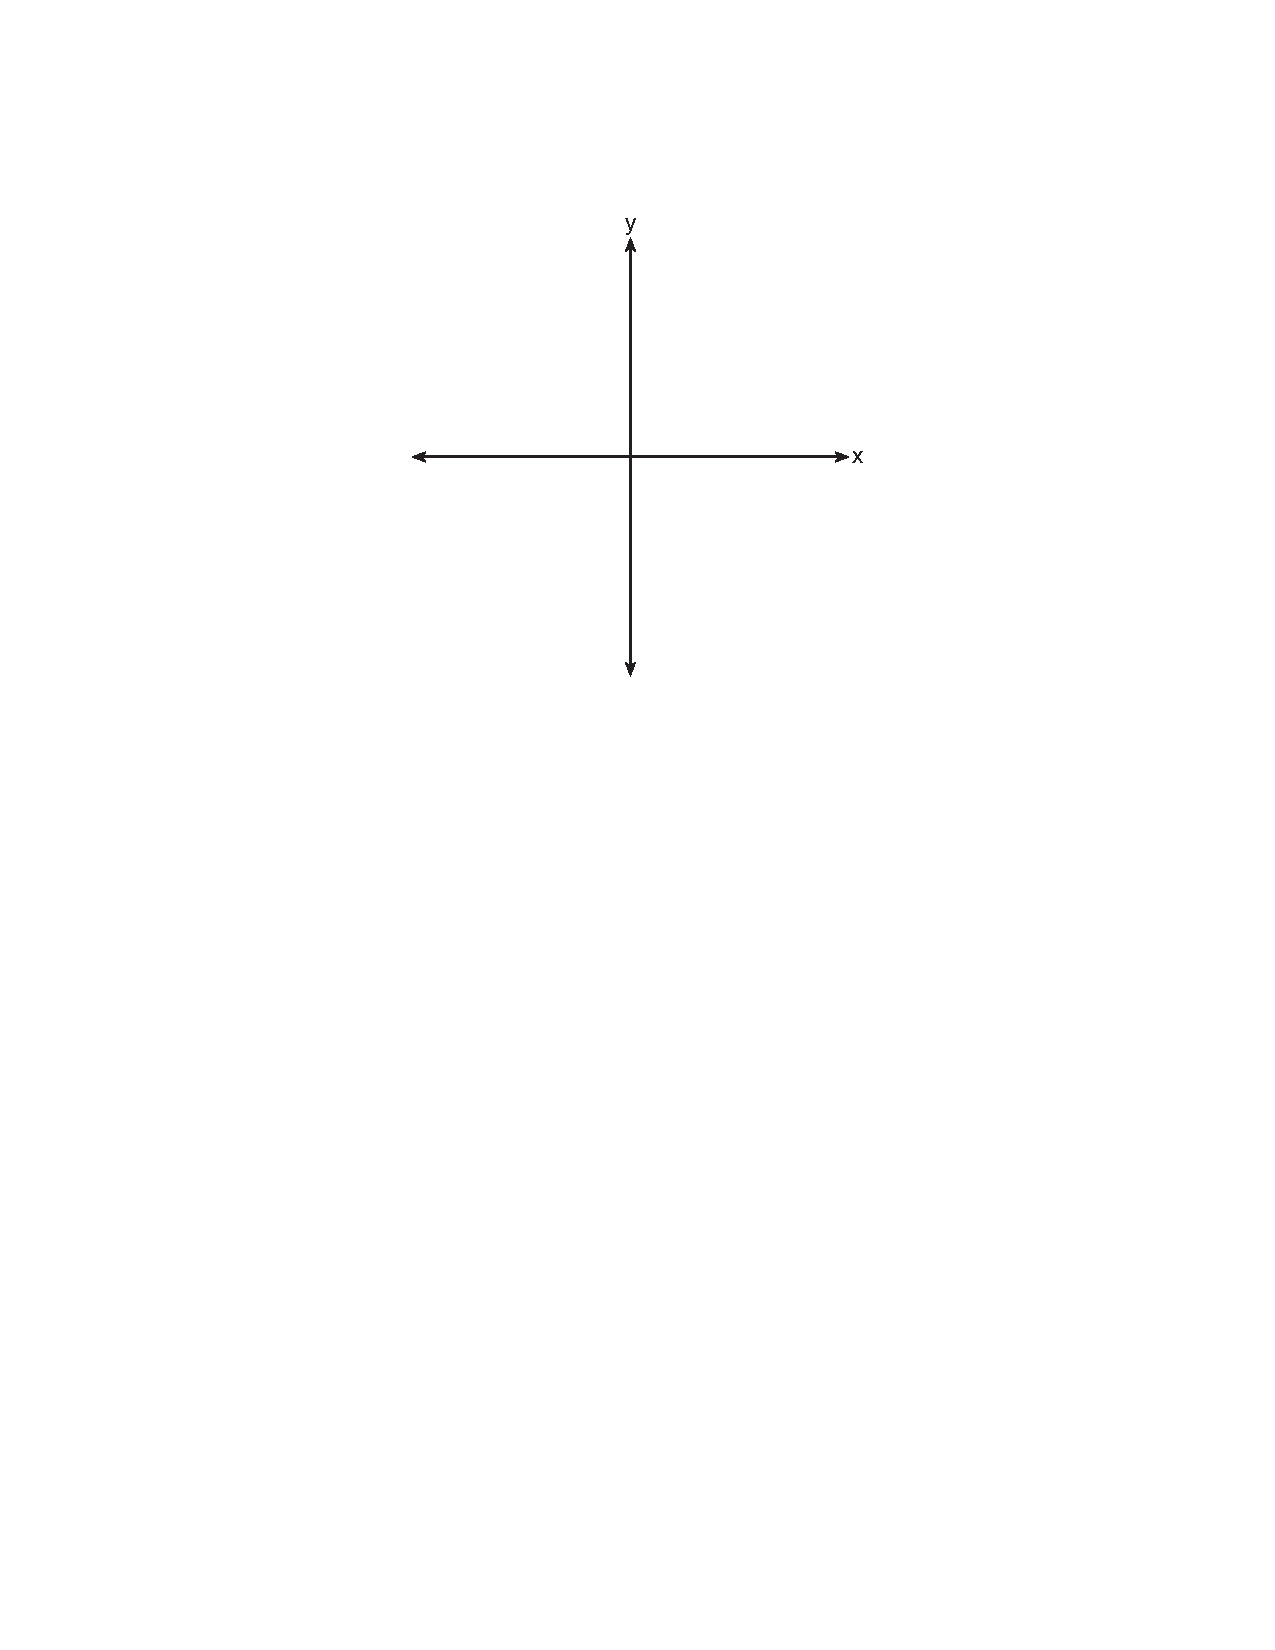
\includegraphics[width=0.5\textwidth]{simple-axes.pdf}
\end{figure}

\newpage %necessary to place the grid following the text
\item  %2 points #29 June 2017
Graph $y =400(.85)^{2x} -6$ on the set of axes below.

\begin{figure}[!ht]
    \centering
    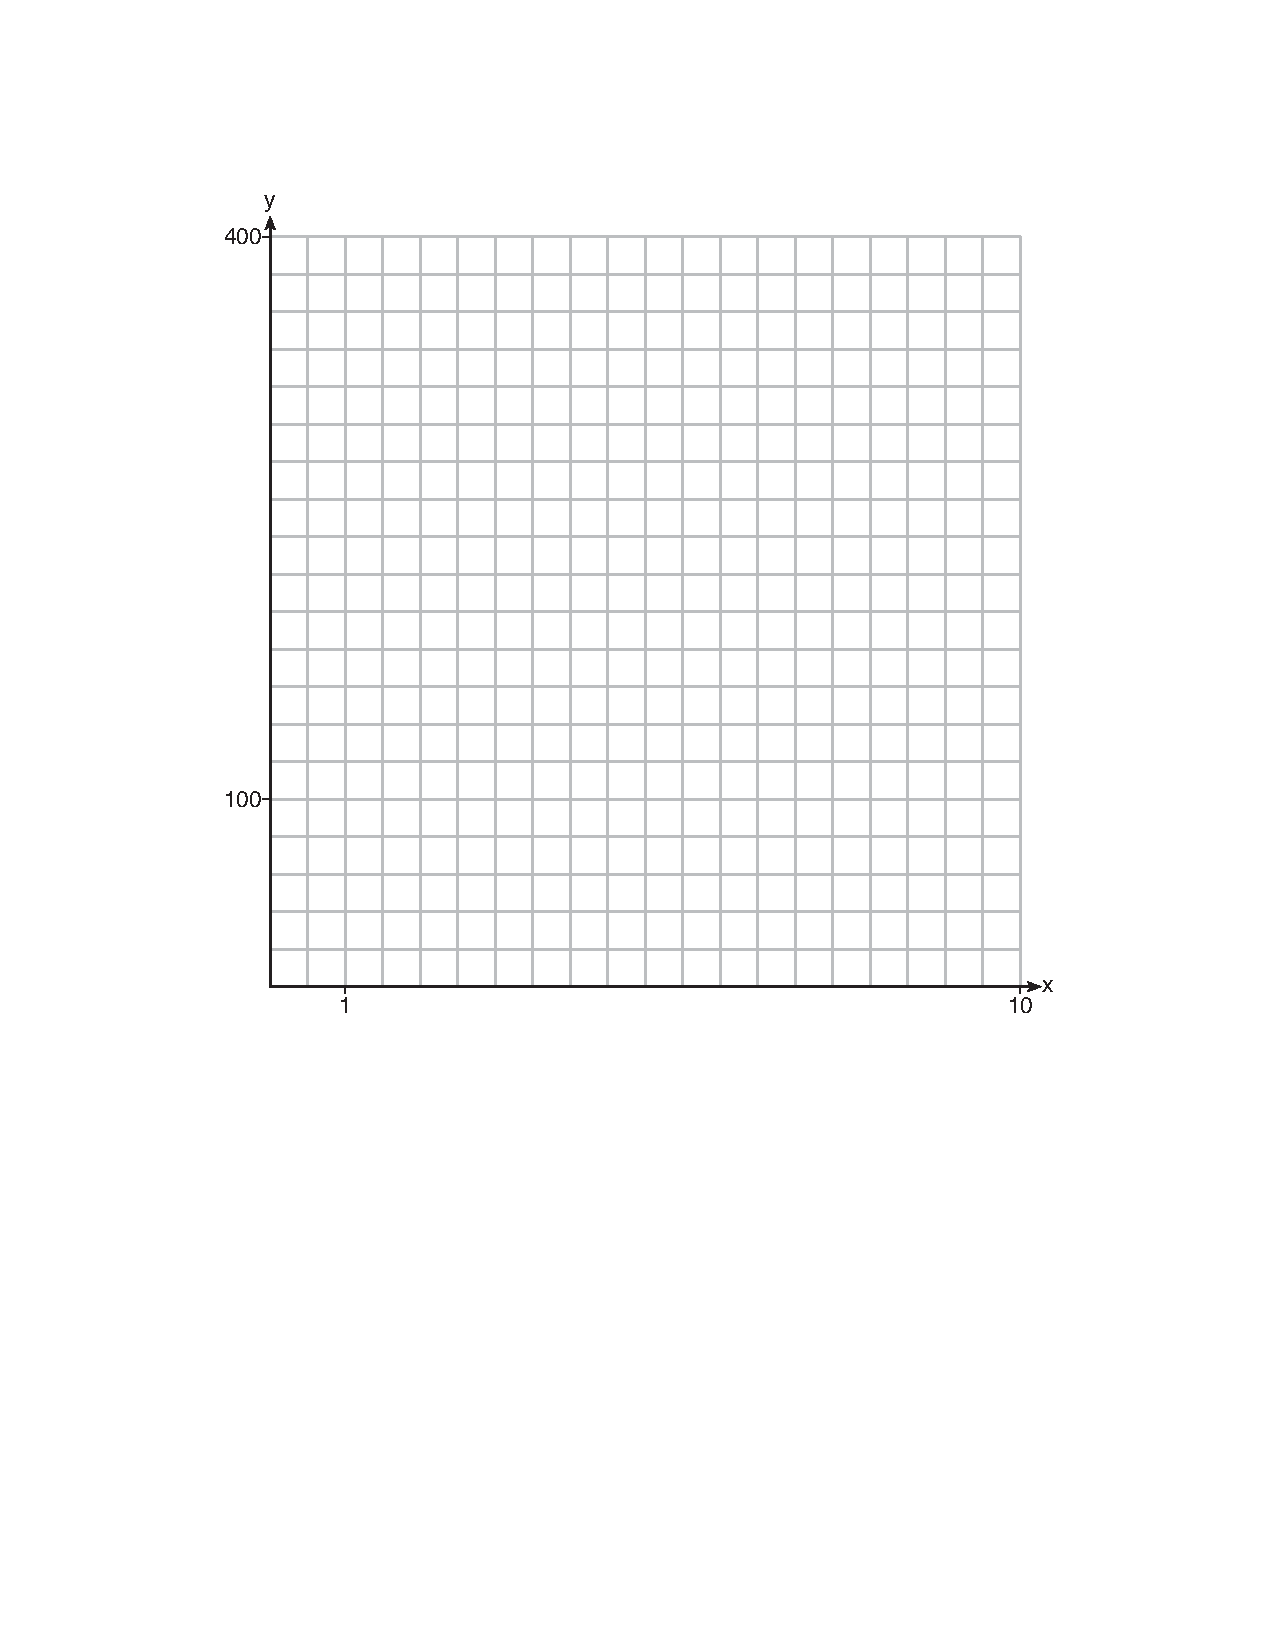
\includegraphics[width=0.85\textwidth]{1stQ-grid-special.pdf}
\end{figure}

\newpage %necessary to place the grid following the text
\item  %4 points #35 June 2017
Graph $y=log_2{(x +3)} - 5$ on the set of axes below. Use an appropriate scale to include \textit{both} intercepts.
\vspace{0.5 in}
\begin{figure}[!ht]
    \centering
    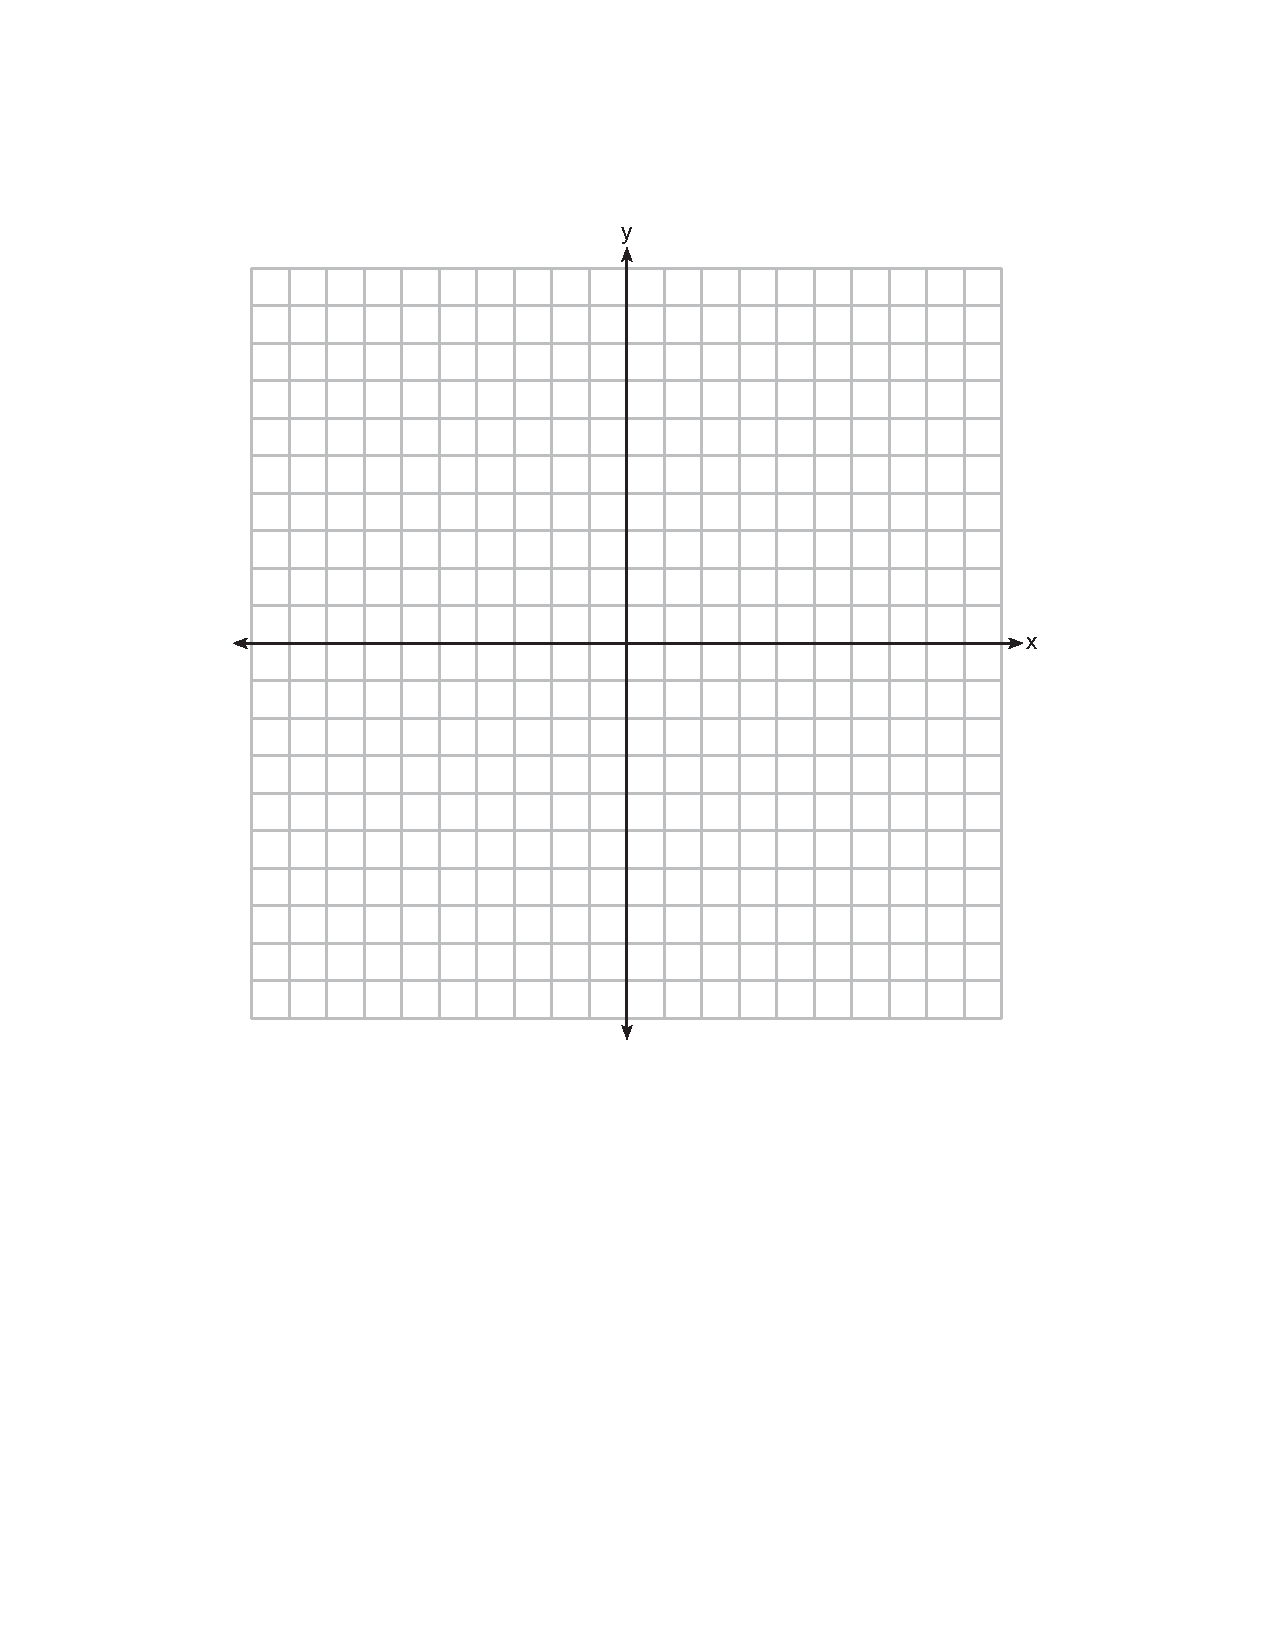
\includegraphics[width=0.75\textwidth]{regents-grid.pdf}
\end{figure}

Describe the behavior of the given function as $x$ approaches $-3$ and as $x$ approaches positive infinity.

\newpage %necessary to place the grid following the text
\item %4 points #35 Aug 2017
\begin{enumerate}
\item  On the axes below, sketch at least one cycle of a sine curve with an amplitude of 2, a mid line at $y = -3/2$, and a period of $2\pi$.

\vspace{0.5 in}
\begin{figure}[!ht]
    \centering
    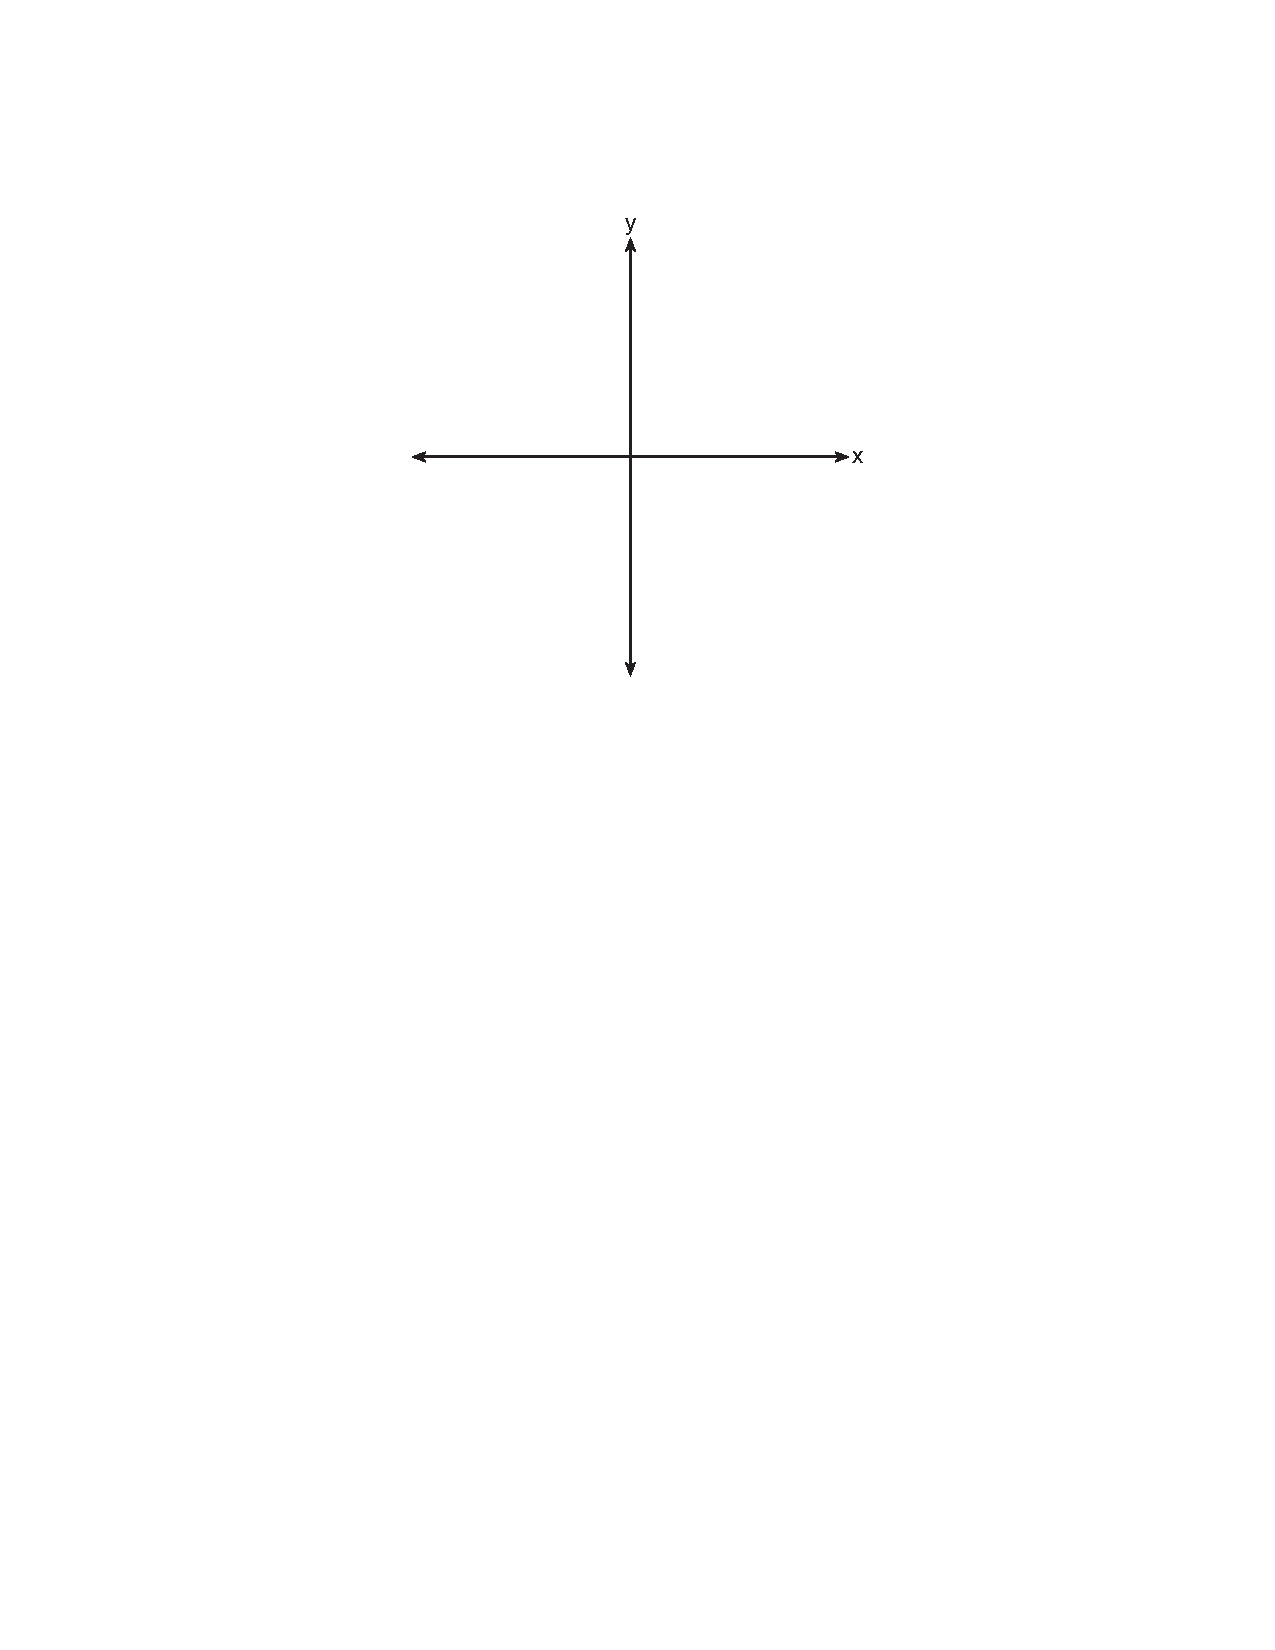
\includegraphics[width=0.65\textwidth]{simple-axes.pdf}
\end{figure}

\item
Explain any differences between a sketch of $\displaystyle y = 2 sin{\left( x - \frac{\pi}{3}\right)} - \frac{3}{2}$ and the sketch from part \textit{a}.
\end{enumerate}

\newpage %necessary to place the grid following the text
\item  %2 points #28 June 2017
The graph below represents the height above the ground, $h$, in inches, of a point on a triathlete’s bike wheel during a training ride in terms of time, $t$, in seconds.

\vspace{0.5 in}
\begin{figure}[!ht]
    \centering
    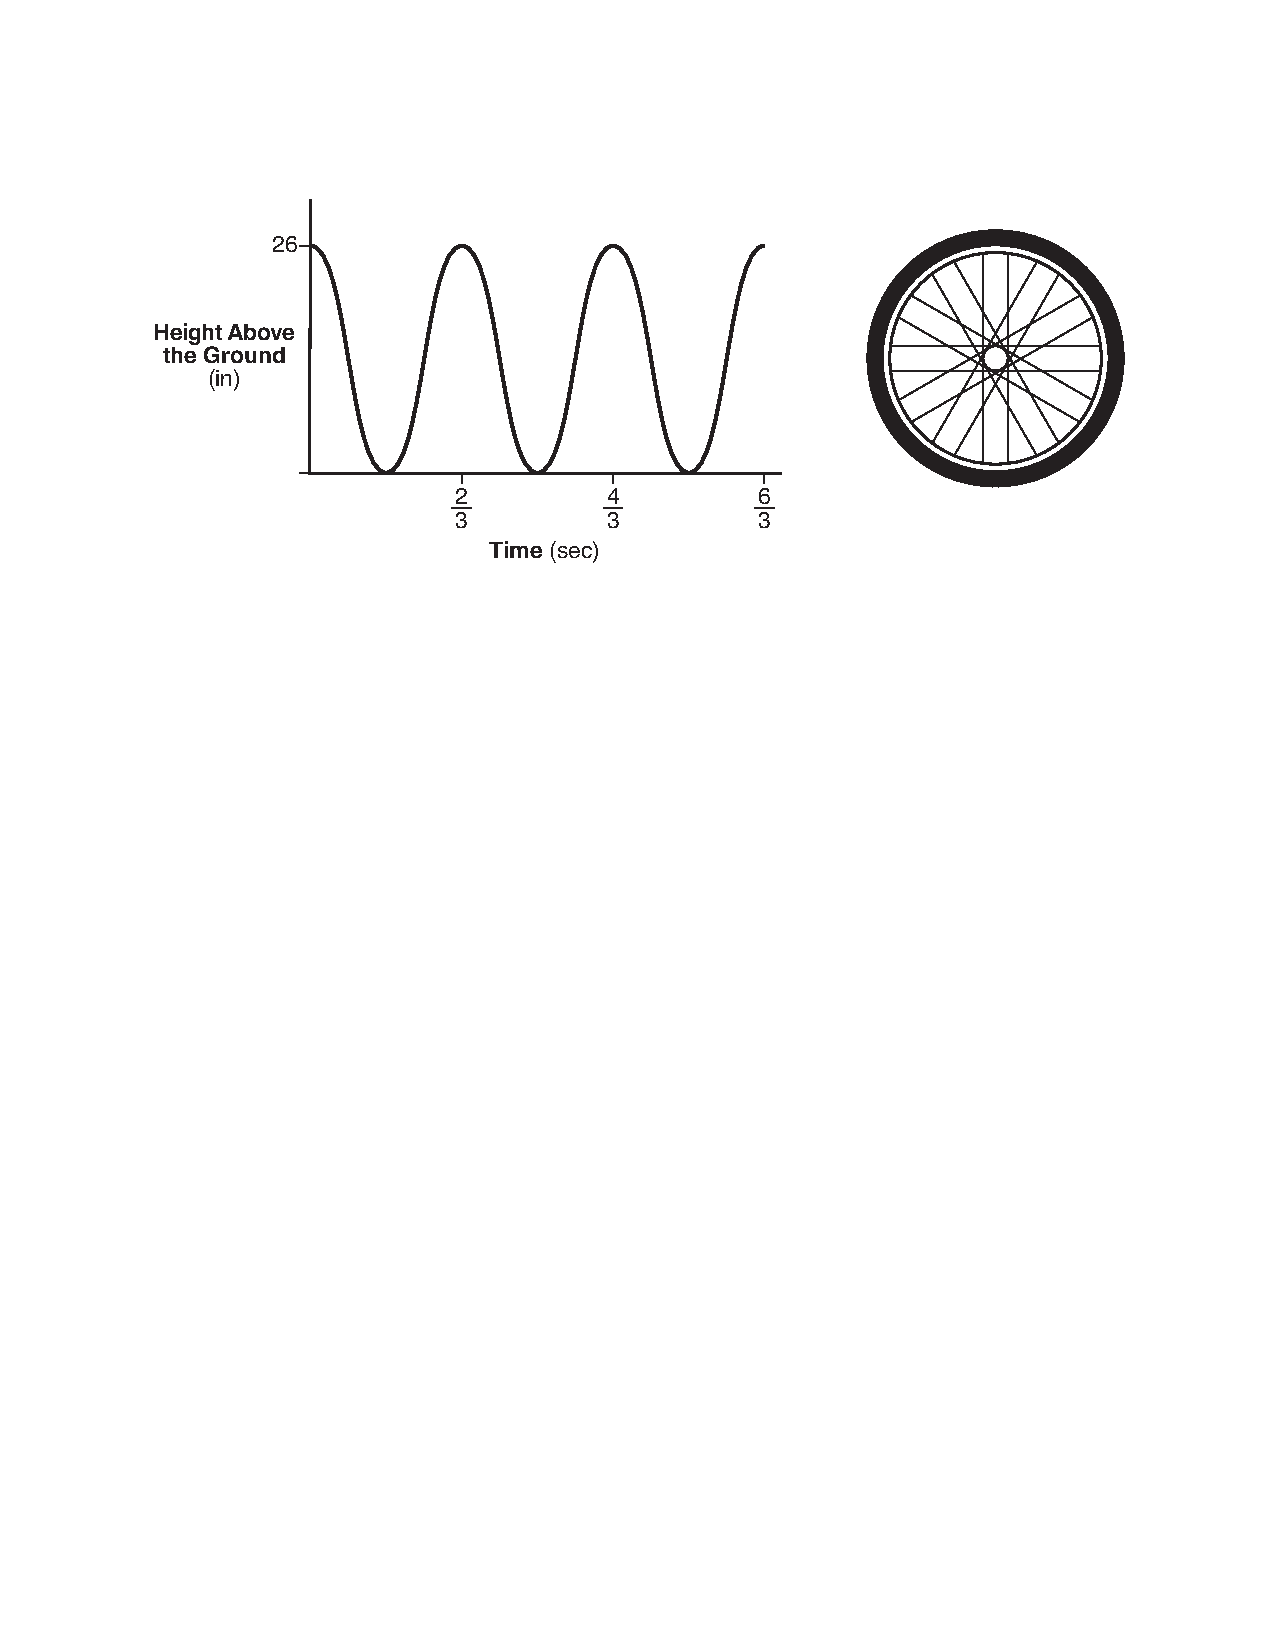
\includegraphics[width=0.85\textwidth]{sine-bike-wheel.pdf}
\end{figure}

Identify the period of the graph and describe what the period represents in this context.